% Chapter 2

\chapter{Survey} % Main chapter title

\label{Chapter2} % For referencing the chapter elsewhere, use \ref{Chapter1} 

\lhead{Chapter 2. \emph{Survey}} % This is for the header on each page - perhaps a shortened title

%----------------------------------------------------------------------------------------

% \emph{Review of relevant literature; review of similar software products or tools.}

\section{Similar applications} % (fold)
\label{sec:similar_applications}

Others have attempted the same task as in this thesis, though with a slightly different approach. Singh et al.~\cite{Singh2011} investigated a ``formulation, where [they] combined the content-based approach with a sentiment analysis task to improve the recommendation results.'' Their approach looks very much like the one taken in this project, but differs in two central ways:

\begin{enumerate}
  \item It uses user reviews from IMDB as content source\footnote{IMDB does not provide open API access at the time of writing.}, and not a more general data source -- as in our case, with Twitter.
  \item It generates recommendations based on genre input.
\end{enumerate}

More generally, much work has been done on sentiment classifying Twitter data. This is elaborated on in section~\ref{sec:the_sentiment_classifier}.

% section similar_applications (end)

%----------------------------------------------------------------------------------------

\section{Twitter data} % (fold)
\label{sec:twitter_data}

Micro-blogging services such as Twitter have enormous amounts of data on almost every topic imaginable. Content is limited in length, and users react to each others' content by ``re-tweeting'', ``favoriting'' or ``replying to'' it. This leaves us with a source of textual data that is:

\begin{description}
  \item[Instant] Users express reactions to events as they experience them.
  \item[Weighted] Users weigh each others' content by interacting with it.
  \item[Concise] Due to limitations on content length, users must express themselves concisely.
\end{description}

The next sections take a look at the ways in which we are able to access this data.

\subsection{Relevant parts of the Twitter API} % (fold)
\label{sub:relevant_parts_of_the_twitter_api}

The various endpoints in the Twitter REST API is divided into 16 categories, spanning everything from search and user timelines to suggested users to follow and spam reporting. A full overview of the available API endpoints is available on Twitter's REST API pages\footnote{\url{https://dev.twitter.com/docs/api/1.1}}.

Of these, only two categories are of relevance to this project, namely \emph{Search} and \emph{OAuth}. The OAuth parts of the API are only relevant as they enable us to search and won't be described any further.

\subsection{The Twitter search API}
\label{ssec:search_api}

The Twitter search API\footnote{\url{https://dev.twitter.com/docs/api/1.1/get/search/tweets}} is a JSON-based REST API, and it takes the following notable parameters:

\begin{description}
  \item[\texttt{q}] \hfill \\
    A UTF-8, URL-encoded search query of 1,000 characters maximum, including operators.
  \item[\texttt{result\_type}] \hfill \\
    Specifies what type of search results you would prefer to receive.
\end{description}

In addition, there are parameters to control the number of messages returned, language, date ranges etc.

\subsubsection{The query parameter}

The \texttt{q} parameter, the search query, is obviously of great importance, as it is the one we primarily will be using to target our search. Apart from the typical boolean operators (AND, OR, and NOT), and the specifying of exact search phrases, it supports the following more domain-specific operators\footnote{A full list of supported operators is available here: \url{https://dev.twitter.com/docs/using-search}}:

\begin{description}
  \item[From/to/referencing user] \hfill \\
    Only return messages from or to a specific user, or that simply mention a specific user somewhere in its message.
  \item[Date ranges] \hfill \\
    Support for ``since'' and ``until'' constraints.
  \item[Other] \hfill \\
    Support for things like only returning messages with links, messages submitted via specific client types, and messages asking a question.
\end{description}

All operators can be combined, and delimiting them by a regular space character serves as an AND clause.

In addition to the previously mentioned operators, the API supports returning tweets matching either a positive or negative sentiment -- a feature which should seem very relevant to the task at hand. However, no information was seemingly available on the mechanics behind it, and after some manual testing it was concluded that it also lacked in its precision.

\subsubsection{The result type parameter}

The other parameter central to our application is the \texttt{result\_type}. It allows us to switch between three possible heuristics for determining which results are returned from the search. We have the choice between three valid values: \texttt{recent}, \texttt{popular}, or \texttt{mixed} -- the latter being a combination of the first two, and also the default.

To know which one to choose, we need to know what constitutes a popular tweet.

% subsection relevant_parts_of_the_twitter_api (end)


\subsection{What constitutes a popular Tweet?}
\label{sub:popular_tweets}

On Twitter, there are several ways of interacting with the system. Terms like ``follow'', ``mention'', ``favorite'', and ``retweet'' are all more or less domain-specific to Twitter, so before moving on -- let's break them down.

\begin{description}
  \item[Follow] \hfill \\
    Users consume each others' content by following each other. The number of followers users have range from 0 to more than 40 million. Following is a one-way relationship, and there is often a big difference in the number of users \emph{following} and \emph{being followed by} a user.
  \item[Reply] \hfill \\
    Users can mention each other in tweets by prepending a username with ``@''. This same mechanism is used to reply to others' content. When replying, the content the Tweet was replying to is stored along with the reply, forming a conversation tree.
  \item[Favorite] \hfill \\
    Users can favorite content, which notifies the content owner and boosts the content in search results etc. It is also trivial to extract all content a particular user has favorited.
  \item[Retweet] \hfill \\
    When a user chooses to retweet another user's content, that content is ``forwarded'' to the user's followers.
\end{description}

One of the greatest benefits of Twitter as a data source is that all these interactions are completely transparent\footnote{Users can make their own content ``private'', but their interactions with other users' non-private content are nonetheless public.}, and can thus be used freely when querying for popular content.


\subsection{Twitter as a Data Source} % (fold)
\label{sub:twitter_as_a_data_source}

There are vast opportunities in managing to understand a data source with the qualities discussed above, but alas -- the diversity and free nature of Twitter as a publishing platform comes at a price: \emph{there is a lot of noise}.
That is not to say that there is little relevant information, but when the service is designed to have such a low threshold for contributing content, a low signal-to-noise ratio seems inevitable.
We will return to the issue of noise in chapter~\ref{sec:evaluation_metrics}, where we try to evaluate correlations between movie titles in our test data and Tweets about the same titles.

This problem of finding content carrying relevant information turns out to perhaps be the biggest challenge of the entire study.

\subsubsection{Novelty of available data} % (fold)
\label{sub:novelty_of_available_data}

As briefly mentioned, part of the hypothesis is that Twitter data is usable for predicting ratings for new content, where collaborative filtering systems perform worse than otherwise.

Novelty, however, is an inherently fundamental quality of Twitter data, even as a data source.
The Twitter search API simply does not expose data more than about a week old.
As it is put in their search API guidelines as of December 2013~\cite{UsingTwitterSearchAPI}, ``The Search API is not [a] complete index of all Tweets, but instead an index of recent Tweets. At the moment that index includes between 6-9 days of Tweets.''

This quality makes Twitter data less than useful when it comes to predicting ratings for movies old enough to have calmed in public debate -- a category which, not surprisingly, includes the vast majority of available movies.

% subsection novelty_of_available_data (end)

% subsection twitter_as_a_data_source (end)

% section twitter_data (end)

\section{The sentiment classifier} % (fold)
\label{sec:the_sentiment_classifier}

Much has already been written on the topic of sentiment analysis of Twitter data~\cite{go2009twitter, go2009twitterdistant, pak2010twitter, agarwal2011sentiment, kouloumpis2011twitter}. This paper, however, is not specifically about improving or analyzing these methods and techniques. What is required is a technique that is good enough to \emph{indicate} the sentiment of \emph{a set of messages}.

For sentiment analysis, I have therefore selected the Twitter sentiment classifier provided by DatumBox, a machine learning SaaS. They provide a broad suite of services within many fields of machine learning. See figure~\ref{fig:datumbox_api} for an overview of their current functionality within the document classification category\footnote{The complete list is currently available at \url{http://www.datumbox.com/api-sandbox/}.}.

Naive Bayes classifiers in general, as well as details regarding the DatumBox implementation, are described in section~\ref{sec:sentiment_analysis_impl}.

\begin{figure}[h]
  \centering
    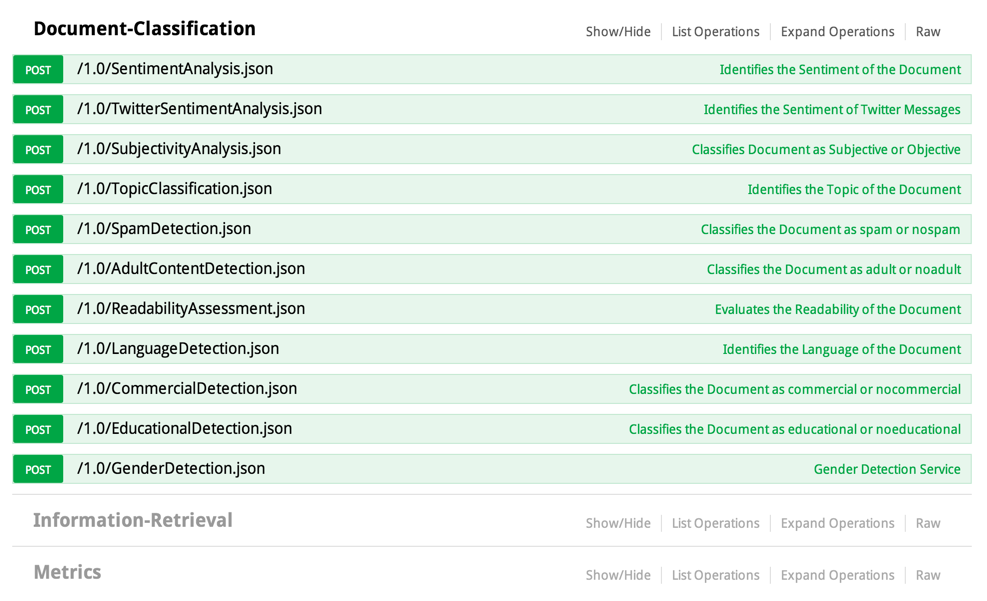
\includegraphics[width=\textwidth]{Figures/datumbox_api}
  \caption{The current endpoints in the DatumBox API in the category ``Document Classification''.}
  \label{fig:datumbox_api}
\end{figure}

\subsection{Alternative approaches}

Two of the most relevant alternatives to the Naive Bayes are SVM and Max Entropy. They are also perfectly capable of performing sentiment classification, and this section will describe them briefly with emphasis on how they perform this task. This is well described in the literature~\cite{pang2002thumbs}, so this survey will not go into great detail.

Max Entropy has been shown to perform several text classification tasks often better than the Naive Bayes, but it also sometimes performs worse~\cite{Nigam99usingmaximum}. The underlying principle of maximum entropy is that without further knowledge, uniform distributions should always be preferred. Training data lay constraints on the distribution, and let us know where the most uniform solutions are.

A Support Vector Machine (SVM) is a large-margin classifier, as opposed to both Naive Bayes and Max Entropy's probabilistic approaches. For a typical two-category case, classifying documents as either positive or negative, SVM attempts to find a hyperplane represented by a vector $\vec{\omega}$ which not only separates the document vectors $\vec{d}$ of one class from the other, but which also maximizes this margin.

Since none of these approaches are particularly dominant in the literature, the simplest solution -- the Naive Bayes classifier provided to us through the DatumBox API -- was chosen.

\section{The Netflix rating dataset}
\label{sec:netflix_dataset}

For evaluating the results, the Netflix rating dataset was used as a benchmark.

The accompanying Readme file descibes the dataset in the following way:

\begin{quote}
  The movie rating files contain over 100 million ratings from 480 thousand
  randomly-chosen, anonymous Netflix customers over 17 thousand movie titles.  The
  data were collected between October, 1998 and December, 2005 and reflect the
  distribution of all ratings received during this period.  The ratings are on a
  scale from 1 to 5 (integral) stars.
\end{quote}

The data used in this work are in two different types of files: one movie metadata file, and many rating files.

The movie metadata file contains an overview of the available movies in CSV format, with lines consisting of the following fields:

\begin{enumerate}
  \item Movie ID
  \item Year of release
  \item Movie title
\end{enumerate}

In a separate directory, 17770 files named by their associated movie ID contain lines of individual ratings, with the following attributes:

\begin{enumerate}
  \item Customer ID
  \item Rating
  \item Date
\end{enumerate}

Unfortunately, the Netflix rating dataset is no longer publicly available, allegedly due to a lawsuit regarding privacy concerns\footnote{\url{http://www.wired.com/threatlevel/2009/12/netflix-privacy-lawsuit/}}.

For more details on how the data was used to evaluate results, see chapter~\ref{Chapter5}.
